\documentclass[12pt,a4paper]{article}

\usepackage{graphicx}% Include figure files
\usepackage{dcolumn}% Align table columns on decimal point
\usepackage{bm}% bold math
%\usepackage{hyperref}% add hypertext capabilities
%\usepackage[mathlines]{lineno}% Enable numbering of text and display math
%\linenumbers\relax % Commence numbering lines

%\usepackage[showframe,%Uncomment any one of the following lines to test 
%%scale=0.7, marginratio={1:1, 2:3}, ignoreall,% default settings
%%text={7in,10in},centering,
%%margin=1.5in,
%%total={6.5in,8.75in}, top=1.2in, left=0.9in, includefoot,
%%height=10in,a5paper,hmargin={3cm,0.8in},
%]{geometry}

\usepackage{multicol}%Para hacer varias columnas
\usepackage{multicol,caption}
\usepackage{multirow}
\usepackage{cancel}
\usepackage{hyperref}
\hypersetup{
    colorlinks=true,
    linkcolor=blue,
    filecolor=magenta,      
    urlcolor=cyan,
}

\setlength{\topmargin}{-1.0in}
\setlength{\oddsidemargin}{-0.3pc}
\setlength{\evensidemargin}{-0.3pc}
\setlength{\textwidth}{6.75in}
\setlength{\textheight}{9.5in}
\setlength{\parskip}{0.5pc}

\usepackage[utf8]{inputenc}
\usepackage{expl3,xparse,xcoffins,titling,kantlipsum}
\usepackage{graphicx}
\usepackage{xcolor} 
\usepackage{nopageno}
\usepackage{lettrine}
\usepackage{caption}
\renewcommand{\figurename}{Figura}
\usepackage{float}
\renewcommand\refname{Bibliograf\'ia}
\usepackage{amssymb}
\usepackage{amsmath}
\usepackage[rightcaption]{sidecap}
\usepackage[spanish]{babel}

\providecommand{\abs}[1]{\lvert#1\rvert}
\providecommand{\norm}[1]{\lVert#1\rVert}
\newcommand{\dbar}{\mathchar'26\mkern-12mu d}

% CABECERA Y PIE DE PÁGINA %%%%%
\usepackage{fancyhdr}
\pagestyle{fancy}
\fancyhf{}

\begin{document}

\begin{enumerate}
    \item \textbf{Investiga el método de la posición falsa para encontrar raíces de una función y a partir del
    programa de la secante (como subrutina) implementa el método}
    
    \begin{verbatim}
PROGRAM secante
!Main program to use the Secant Method to find the root of
! f(x)=exp(x)*ln(x)-x*x=0.
!
REAL*8 :: DL,A,B,DX,X0,H,C
INTEGER :: ISTEP
 C = 0.0
 DL = 1.0D-15
 A = 1.0
 B = 2.0
 DX = (B-A)/10.0
 X0 = (A+B)/2.0
 PRINT*,'X0=',X0
 CALL SECANT (DL,X0,DX,ISTEP)
 PRINT*, ISTEP,X0,DX
 DX = (B-A)/10.0
 CALL FP (A,B,C,DX,DL,ISTEP)
 PRINT*, ISTEP,C,DX
END PROGRAM SECANTE
!
 SUBROUTINE SECANT (DL,X0,DX,ISTEP)
!
! Subroutine for the root of f(x)=0 with the secant method.
!
 IMPLICIT NONE
 INTEGER, INTENT (INOUT) :: ISTEP
 REAL*8, INTENT (INOUT) :: X0,DX
 REAL*8 :: X1,X2,D,F,FX
 REAL*8, INTENT (IN) :: DL
 PRINT*, 'DX=',DX,'X0=',X0, DL
 ISTEP = 0
 X1 = X0 + DX
 DO WHILE (DX.GT.DL)
 D = F(X1) - F(X0)
 X2 = X1 - F(X1)*(X1-X0)/D
 X0 = X1
 X1 = X2
 DX = ABS(X1 - X0)
 ISTEP = ISTEP + 1
 ENDDO
 END SUBROUTINE SECANT
!
 SUBROUTINE FP(A,B,C,DX,DL,ISTEP)
 IMPLICIT NONE
 INTEGER, INTENT (INOUT) :: ISTEP
 REAL*8, INTENT (IN) :: A,B,DL
 REAL*8 :: F,X,Y
 REAL*8, INTENT (INOUT) :: C,DX
 X=B
 Y=A
 ISTEP=0
 DO WHILE (DX.GT.DL)
  ISTEP=ISTEP+1
  C=(F(X)*Y-F(Y)*X)/(F(X)-F(Y))
  IF (F(A)*F(C).LT.0) THEN
   X=C
   DX=ABS(Y-C)
  ELSE
   Y=C
   DX=ABS(X-C)
  END IF
 END DO
 END SUBROUTINE FP
!
 FUNCTION F(X)
 IMPLICIT NONE
 REAL*8 :: F 
 REAL*8, INTENT (IN) :: X
 F = EXP(X)*LOG(X) - X*X
 END
    \end{verbatim}
    
    \begin{figure}[h]
        \centering
        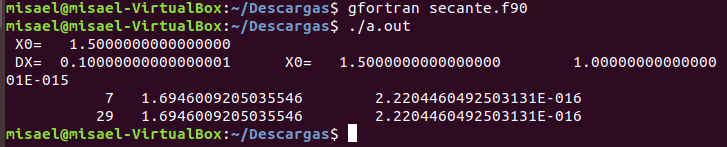
\includegraphics[scale=0.8]{1.PNG}
    \end{figure}
    
    El método  de la posición falsa tarda poco más de 4 veces que el método de la secante lo que es bastante 

    \item \textbf{Haz un programa que haga distintas aproximaciones (h}$\rightarrow$\textbf{0) a la derivada de una función que conozcas utilizando la precisión “extra” que hemos visto para un valor determinado
    comparando con el resultado exacto. ¿cuál es la mejor h?}
    
    \begin{verbatim}
PROGRAM derivada
IMPLICIT NONE
INTEGER :: i
INTEGER, PARAMETER :: extra = SELECTED_REAL_KIND(p=24,r=1000)
REAL(extra) :: x,hh,xx,dif,ff
WRITE(*,*) "x=7.1"
WRITE(*,*) "f(x)=x**(1/2)"
WRITE(*,*) "f'(x)=1/2*sqrt(x)"

x=7.1_extra
xx= 1/(2*SQRT(x))

WRITE(*,*)"           ", "i/h", "      ", "f'(x)", "         ", "f'(x)(approx)", "      ", "|f'-sqrt(x)/sqrt(x)|"

DO i=1,24
 WRITE(*,*) i
 hh=1._extra/10._extra**i
 ff=(SQRT(x+hh)-SQRT(x))/hh 
 dif=ABS((ff-xx)/xx)
 PRINT 10,hh ,xx,ff, dif
10 FORMAT(2X,6F16.13)
END DO

END PROGRAM derivada
    \end{verbatim}
    
    \begin{figure}[h]
        \centering
        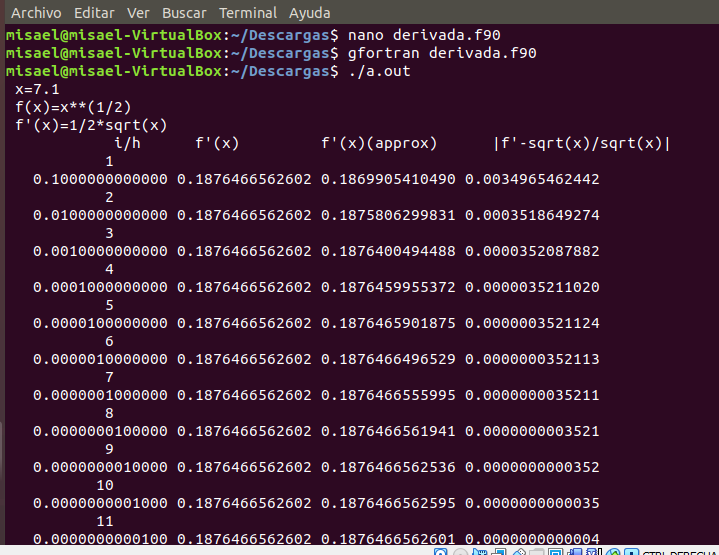
\includegraphics[scale=0.8]{2.1.PNG}
    \end{figure}
    
    \begin{figure}[h]
        \centering
        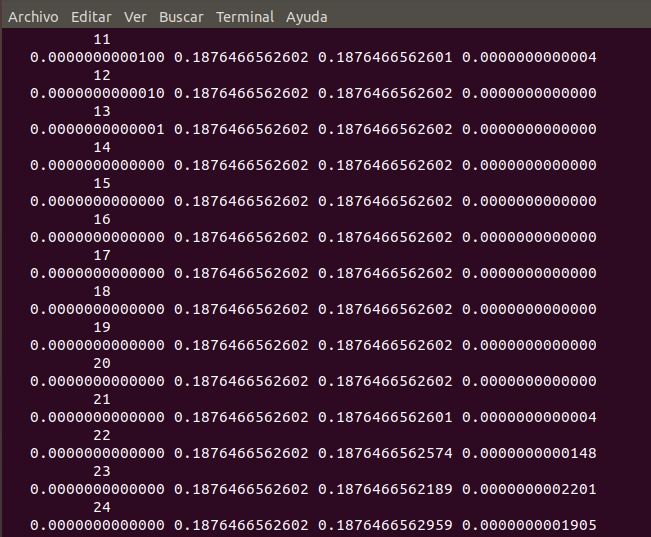
\includegraphics[scale=0.8]{2.2.PNG}
    \end{figure}
    
    El mejor valor de h debe estar entre $1/10^{11}$ y $1/10^{21}$, intenté usar mayor precisión para los decimales pero el programa regresaba puros asteriscos :(
    

    \item \textbf{Haz un programa que rote una imagen en formato .bmp 180 grados. El problema se reduce
    a cambiar (en tono de grises) el primer píxel por el último, el segundo por penúltimo, el tercero
    por el antepenúltimo, el cuarto...y así hasta llegar a la mitad, ¿verdad? (ver videos de arreglos)}
    
    \begin{verbatim}
PROGRAM ROTACION

IMPLICIT NONE
CHARACTER*30 :: NOM1,NOM2
INTEGER :: NTAM,NL,NA,NPIX,NEN,i
INTEGER*1, ALLOCATABLE, DIMENSION(:) :: x,y


WRITE(*,*) "Indica el nombre del archivo de imagen"
READ(*,*) NOM1
!NOM1 = "gato.bmp"

WRITE(*,*) "Indica el nombre de archivo rotado"
READ(*,*) NOM2

WRITE(*,*) "Escribe el tamaño en bytes"
READ(*,*) NTAM
!NTAM = 172854

WRITE(*,*) "Indica el largo de la imagen en pixeles"
READ(*,*) NL
!NL = 180

WRITE(*,*) "Indica el alto de imagen en pixeles"
READ(*,*) NA
!NA = 320

WRITE(*,*) "Indica el numero de bytes por pixel"
READ(*,*) NPIX
!NPIX = 3

ALLOCATE(x(NTAM),y(NTAM))

OPEN(1,FILE=NOM1,ACCESS="DIRECT",FORM="UNFORMATTED",STATUS="OLD",RECL=NTAM)!abre la imagen a rotar
READ(1,REC=1)(x(i),i=1,NTAM)
NEN = NTAM - NL*NA*NPIX

DO i = 1,NEN !copia el encabezado
 y(i)=x(i)
END DO

DO i = NEN+1,NTAM !intercambia los pixeles para rotar 180 grados
  y(i) = x(NTAM-i+NEN)
END DO

OPEN(2,FILE=NOM2,ACCESS="DIRECT",FORM="UNFORMATTED",STATUS="NEW",RECL=NTAM) !abre la imagen rotada
WRITE(2,REC=1)(y(i),i=1,NTAM)

CLOSE(1)
CLOSE(2)

END PROGRAM ROTACION
    \end{verbatim}
    
    \begin{figure}[h]
        \centering
        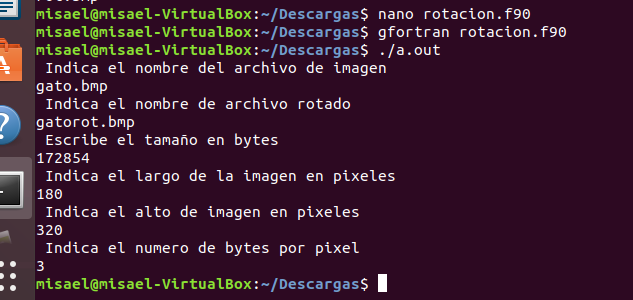
\includegraphics[scale=0.8]{3.1.PNG}
    \end{figure}
    
    Las imágenes original y rotada se pueden ver a continuación, por alguna razón que aun no entiendo la imagen rotada se hizo un poco rojiza pero parece estar bien
    
    \begin{figure}[h]
        \centering
        
\includegraphics[scale=1]{gato.png}
    \end{figure}
    
    \begin{figure}[h]
        \centering
        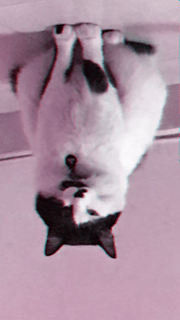
\includegraphics[scale=1]{gatorot.png}
    \end{figure}
\end{enumerate}

\end{document}
